\documentclass{article}
\usepackage{multimedia}
\usepackage{polski}
\usepackage[utf8]{inputenc}
\usepackage[T1]{fontenc}
\usepackage{color}
\usepackage{amsthm}
\usepackage{graphicx}
\usepackage{float}
\usepackage{afterpage}
\usepackage[labelsep=period]{caption}

\renewcommand*{\figurename}{Rysunek}
\renewcommand{\thefigure}{\arabic{figure}}
\renewcommand*{\tablename}{Tabela}
\renewcommand{\thetable}{\arabic{figure}}
\renewcommand*{\thesection}{\arabic{section}.}
\renewcommand*{\thesubsection}{\arabic{section}.\arabic{subsection}.}


\begin{document}

\begin{titlepage}
	\vspace{2em}{\centering\large{Instytut Informatyki Uniwersytetu Wrocławskiego}\par}

  \vspace{17em}{\centering\large{Agnieszka Dudek, Piotr Kowalczyk}\par}

	\vspace{2em}{\centering\huge{Dokumentacja projektu \textit{Tablica efektów kształcenia}}\par}

	\vspace{4em}{\centering\Large{Koncepcja wykonania systemu}\par}

	\vspace{17em}{\centering\large{Wrocław, \today}\par}

	\vspace{1em}{\centering\large{Wersja 0.5}\par}

\end{titlepage}

\addtocounter{page}{1}
\newpage

\begin{table}[h!]
	\begin{center}
		\caption{Historia zmian dokonywanych w dokumencie}
		\begin{tabular}{|l|l|l|l|}
			\hline
			Data & Numer wersji & Opis & Autor \\
			\hline \hline
			2018-11-26 & 0.1 & Utworzenie dokumentu & Piotr Kowalczyk \\
			\hline 
			2018-12-01 & 0.2 & Korekta dokumentu & Agnieszka Dudek \\
			\hline
			2018-12-04 & 0.3 & Korekta punktów 4.1 i 4.2 & Agnieszka Dudek \\
			\hline
			2018-12-05 & 0.4 & Korekta dokumentu & Piotr Kowalczyk \\
			\hline
			2018-12-13 & 0.5 & Korekta dokumentu & Agnieszka Dudek \\
			\hline			
    \end{tabular}
	\end{center}
\end{table}	

\tableofcontents

\newpage


\section{Wprowadzenie}

\subsection{Cel dokumentu}
Niniejszy dokument ma na celu precyzyjny opis koncepcji wykonania projektu Tablica efektów kształcenia.
Dokument jest drugim z listopadowej grupy zadań realizowanych w ramach pracowni z inżynierii oprogramowania.

\section{Scenariusze przypadków użycia}
Dla trzech historyjek użytkownika przedstawionych w dokumencie \textit{Specyfikacja wymagań} opisujemy dokładne scenariusze dialogu człowieka z komputerem.

\subsection{Pierwszy scenariusz}
Po otwarciu sesji w Systemie Zapisów widoczny jest \textbf{przycisk} o nazwie Tablica efektów (dalej zwany przyciskiem). 
Znajduje się on za przyciskami \textsf{Pracownicy} i \textsf{Studenci}. Po kliknięciu przycisku wyświetla się ekran, na którym znajdują się:
\begin{itemize}
	\item lista dotychczas zrealizowanych efektów kształcenia,
	\item lista efektów kształcenia czekających na zrealizowanie,
	\item lista punktów ECTS zdobytych z poszczególnych grup przedmiotów.
\end{itemize}
Student może skupić uwagę na trzeciej z wymienionych list lub wydrukować wszystkie dane.

\subsection{Drugi scenariusz}
Analogicznie do pierwszego scenariusza po kliknięciu przycisku Tablica efektów wyświetlone zostają listy zrealizowanych i niezrealizowanych efektów kształcenia.
Studentka może przewijać listę efektów kształcenia czekających na zrealizowanie i sprawdzić, czy uda jej się spełnić wszystkie wymagania w kolejnym semestrze.

\subsection{Trzeci scenariusz}
Zmiana statusu przedmiotu w USOS powoduje, że podczas następnej migracji danych aktualizowane są dane w Systemie Zapisów dotyczące efektów kształcenia.


\afterpage{\null\newpage}
\newpage


\section{Projekty ekranów związanych z przypadkami użycia}
\subsection{Pierwszy scenariusz}
\begin{figure}[H]
	\begin{center}
		
\includegraphics[scale=0.45]{te.png}
		\caption{Projekt przycisku Tablica efektów}
	\end{center}
\end{figure}

\begin{figure}[H]
	\begin{center}
		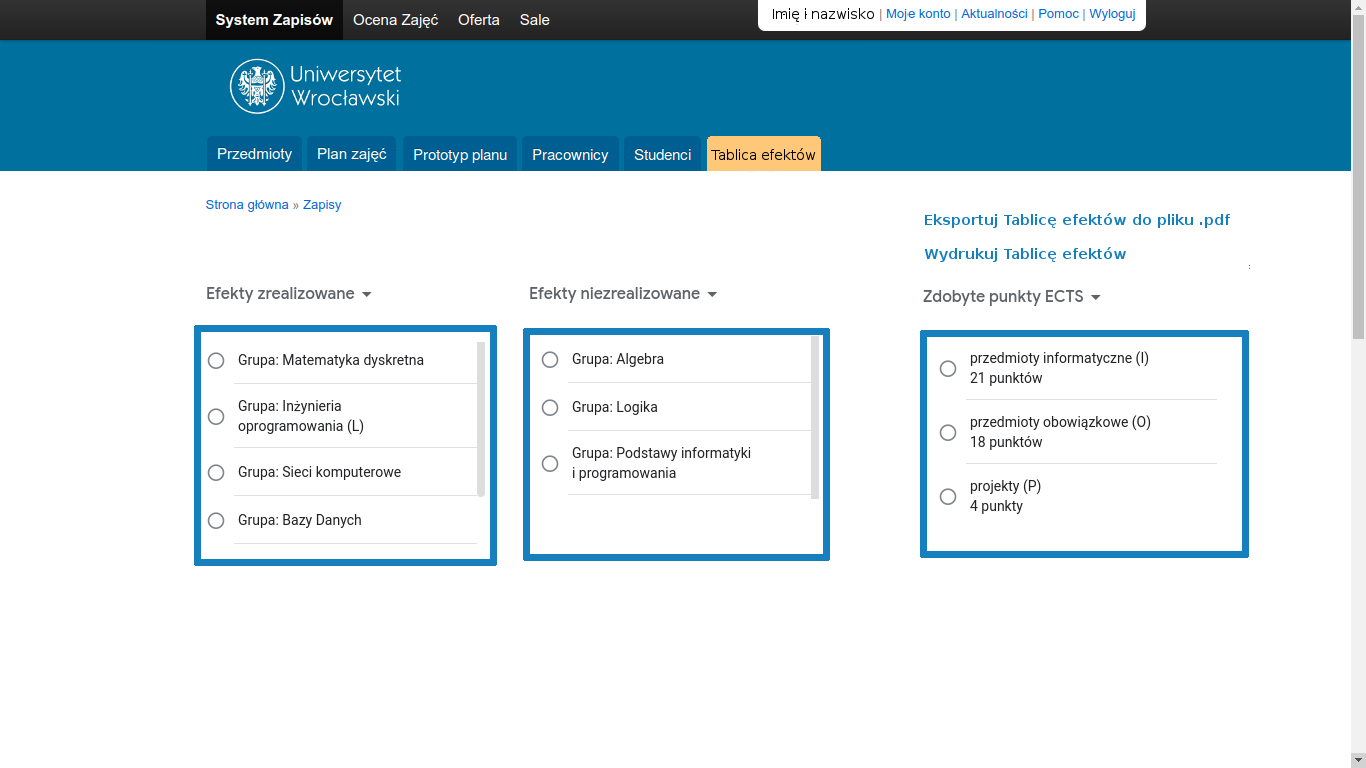
\includegraphics[scale=0.23]{tabl.png}
		\caption{Projekt list zrealizowanych efektów}
	\end{center}
\end{figure}

\subsection{Drugi scenariusz}
\begin{figure}[H]
	\begin{center}
		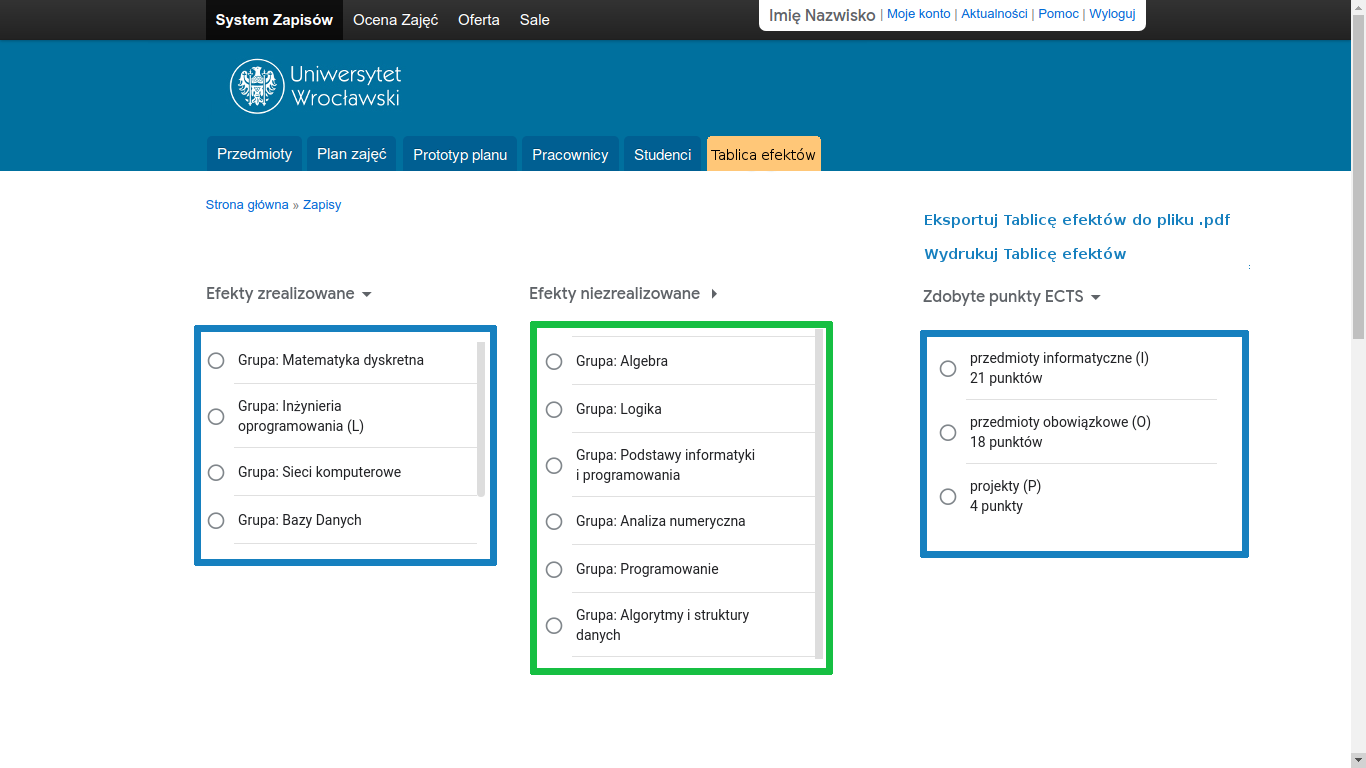
\includegraphics[scale=0.23]{rozwin.png}
		\caption{Projekt rozwijania poszczególnych list}
	\end{center}
\end{figure}

\subsection{Trzeci scenariusz}
\begin{figure}[H]
	\begin{center}
		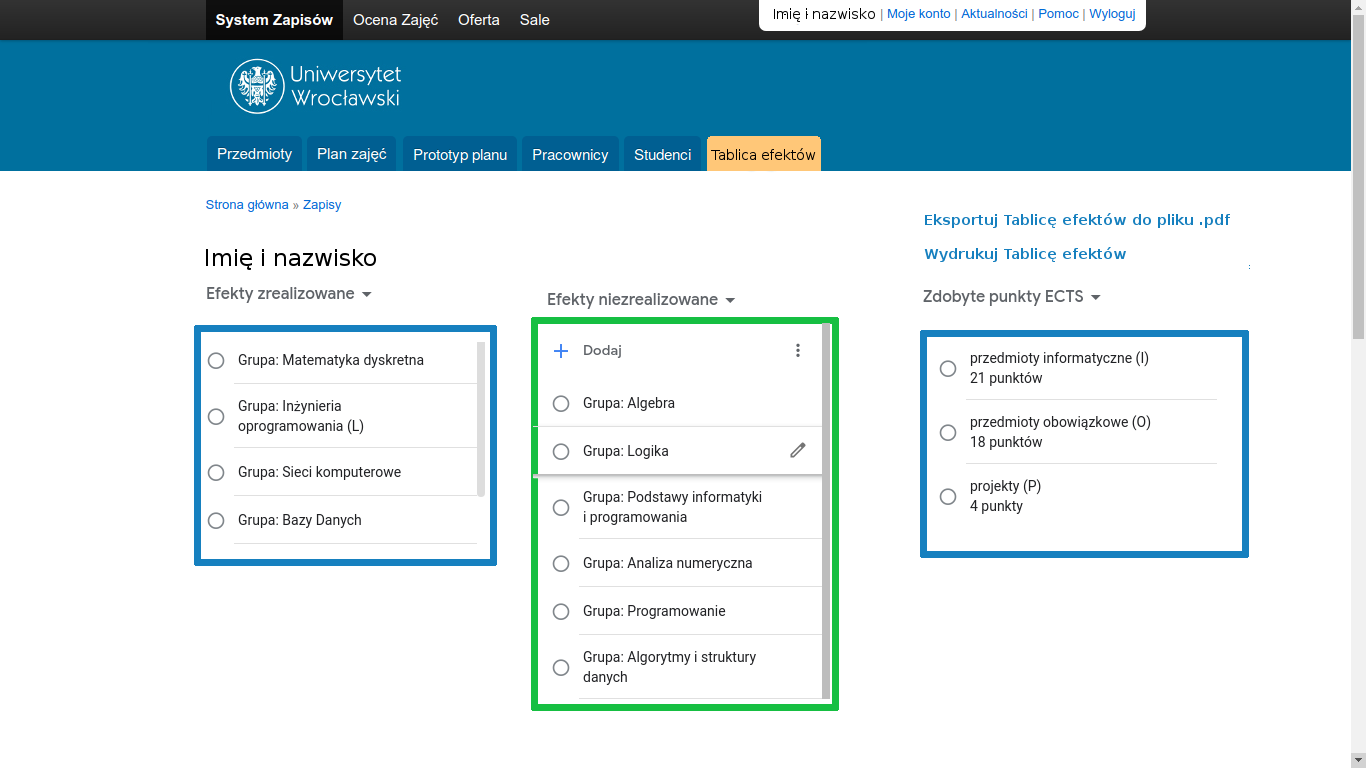
\includegraphics[scale=0.23]{edycja.png}
		\caption{Projekt list w trybie ręcznego redagowania}
	\end{center}
\end{figure}


\section{Projekt architektury}

\subsection{Model konceptualny rzeczywistości, której dotyczy nasza aplikacja}
Obiekty świata rzeczywistego:
\begin{itemize}
 \item student [imię, nazwisko, numer indeksu, tok studiów],
 \item efekt kształcenia [nazwa, tok studiów, status realizacji],
 \item grupa przedmiotów [nazwa, tok studiów, liczba zdobytych punktów].
\end{itemize}
Związki binarne o typie asocjacji 1:M\,:
\begin{itemize}
 \item student posiada efekt kształcenia [do wyboru ze strony studenta],
 \item student zbiera punkty w grupie przedmiotów [obowiązkowe ze strony studenta].
\end{itemize}

\subsection{Podstawowe cechy aplikacji}
\begin{itemize}
 \item aplikacja będzie częścią oprogramowania System Zapisów,
\begin{figure}[H]
	\begin{center}
		
\includegraphics[scale=0.3]{syst.png}
	\end{center}
\end{figure}
 \item aplikacja będzie używać bazy danych,
 \item aplikację napiszemy z użyciem zintegrowanego środowiska programistycznego Eclipse,
 \begin{figure}[H]
	\begin{center}
		
\includegraphics[scale=0.12]{eclipse.png}
	\end{center}
\end{figure}
 \item aby przetestować aplikację, skorzystamy z oprogramowania TestRail.
 \begin{figure}[H]
	\begin{center}
		
\includegraphics[scale=0.2]{testrail.png}
	\end{center}
\end{figure}
\end{itemize}


\subsection{Omówienie interfejsów systemu z otoczeniem}
System będzie posiadać trzy interfejsy.
Głównym interfejsem będzie strona Systemu Zapisów.
Drugim, równie ważnym, będzie sprzęgnięcie systemu z USOS.
Poza tym system musi umożliwić ręczną modyfikację danych w sytuacjach wyjątkowych (np. nieskorelowanych ze zmianami w USOS).


\section{Schemat bazy danych}
Baza danych składa się z tylu tablic, ile jest toków studiów na kierunku informatyka na naszej uczelni (nie można realizować jednocześnie dwóch toków studiów).
Kluczami są identyfikatory studentów, a efekty kształcenia kolejnymi polami typu boolean lub integer.

Baza jest tworzona (za pierwszym razem) i aktualizowana podczas migracji danych z USOS.


\section{Zasady kodowania}
Podczas kodowania będą obowiązywać zasady obowiązujące w Systemie Zapisów, a przypadki niezdefiniowane będą rozstrzygane zgodnie z normą wypracowaną przez Google\footnote{Zob. https://google.github.io/styleguide/jsguide.html.}.


\newpage


\section{Ryzyko}

\subsection{Identyfikacja ryzyka}
Nie musimy się bać, że nasze oprogramowanie przestanie być potrzebne. Nie musimy się bać, że stracimy odbiorców. Ale wykonanie projektu może się opóźnić i to jest główne ryzyko.
Musimy również pokazać naszym odbiorcom, że jesteśmy wiarygodni. Nasze dane od początku muszą być kompletne i prawdziwe, w przeciwnym wypadku stracimy zaufanie studentów.

\subsection{Zasady zarządzania ryzykiem}
Aby zapewnić kompletność danych, musimy skonsultować się z osobami odpowiedzialnymi za system efektów kształcenia na naszej uczelni oraz pracownikami dziekanatu, którzy odpowiadają za aktualizowanie danych.
Ważne jest również dogłębne przetestowanie naszego produktu, aby mieć pewność, że wyświetlane dane są zawsze poprawne.

Żeby zdążyć z projektem do końca semestru letniego, musimy trzymać się harmonogramu od początku realizacji projektu. 
Dodatkowo już na początku możemy skontaktować się z osobami, na których konsultacjach będzie nam zależało.


\section{Ocena zgodności wykonanych prac z planami}
Ostatnim etapem pracy będzie porównanie osiągniętych efektów z planami.
Głównym celem naszego projektu jest dostarczanie danych o zrealizowanych efektach kształcenia.
Dopuszczamy zmianę ostatecznego wyglądu strony oraz podziału informacji na listy, jednak nie możemy zmienić zakresu wyświetlanych danych.


\end{document}
